\section{Agent Architecture}
\subsection{Decision Loop and Task Code Generation}
Auto-ORCA translates natural-language requests into scientific objectives, computational conditions, and executable plans.
The model proposes parameters, Python programs, or ORCA input based on the available evidence; the software checks dependencies, permissions, and resources before execution.
New results are read, checked, and evaluated against the objectives before being returned to the next decision cycle.
Figure~\ref{fig:architecture} presents the overall architecture.
Both successful calculations and failure information enter the feedback loop, and the system does not prescribe a fixed sequence of optimization, frequency, and single-point calculations.

\begin{figure}[htbp]
  \centering
  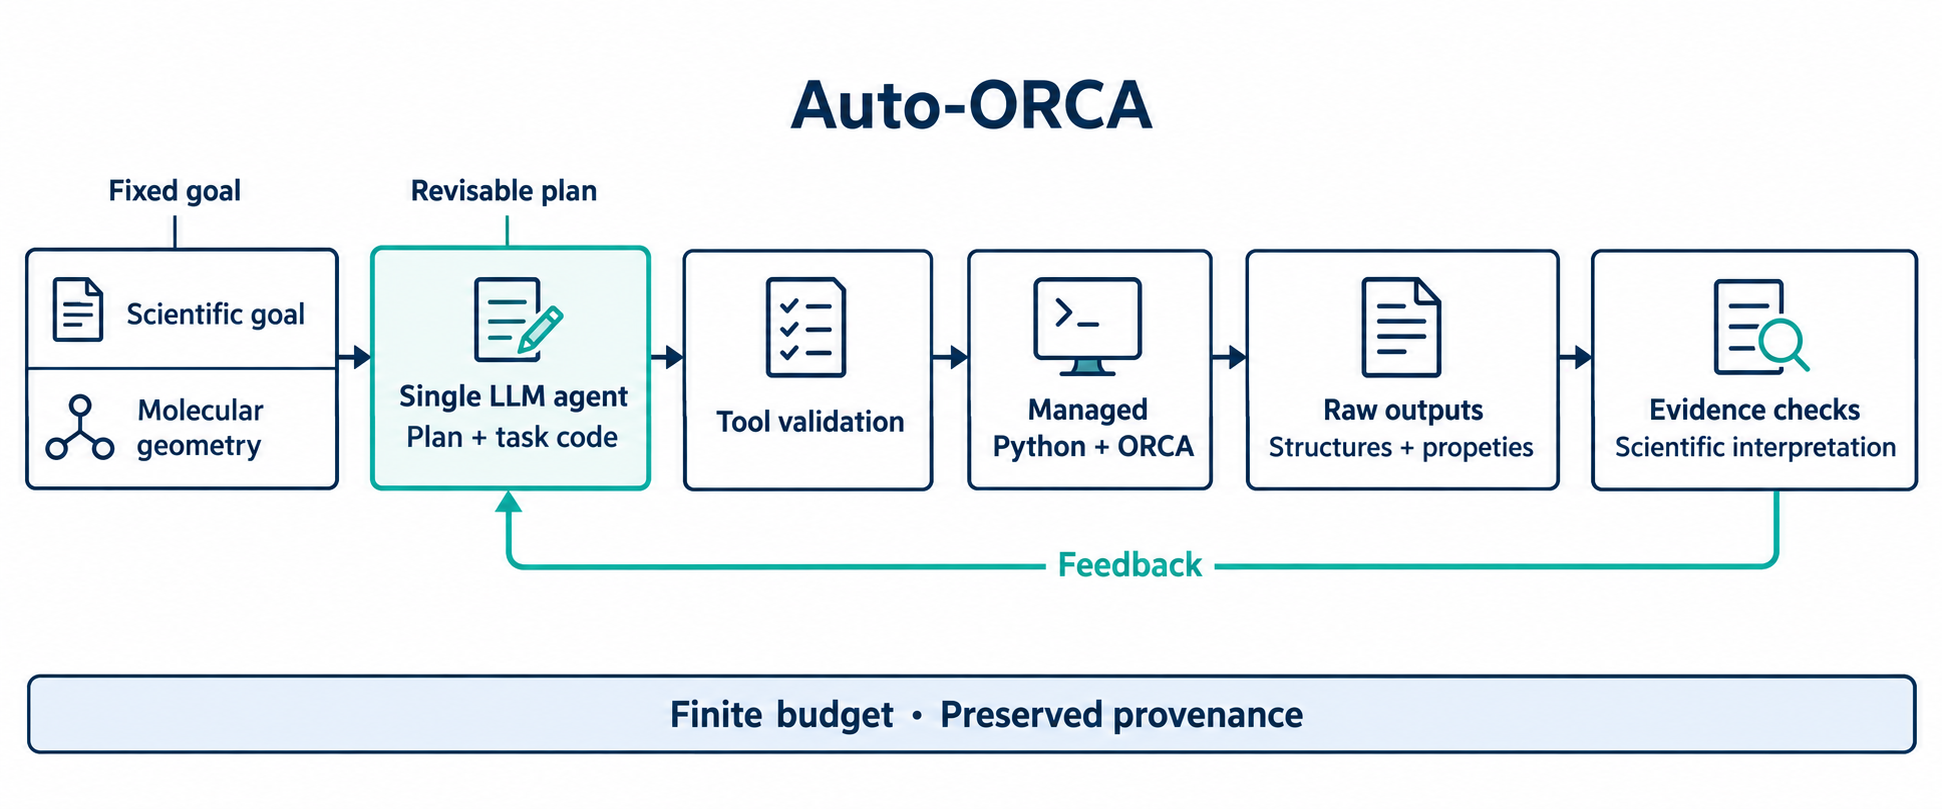
\includegraphics[width=\linewidth]{auto-orca-architecture.png}
  \caption{The single decision loop in Auto-ORCA.
  The original objectives and minimum evidence requirements constrain result evaluation.
  The model uses generic tools to organize managed Python and ORCA execution and revises the plan in response to the returned evidence.}
  \label{fig:architecture}
\end{figure}

Task-specific algorithms are expressed in generated code, while generic tools handle input validation, execution, and artifact management.
For example, a program may construct a finite set of geometries, request an energy calculation for each, and compare the results in consistent units.
OPI input, native ORCA input, and calculation requests issued within Python share the same execution entry point~\cite{opi}.
The thin interface returns execution receipts and raw artifacts without embedding an implicit solution algorithm for an individual problem.
This design allows the same tools to support different tasks while maintaining explicit execution boundaries.

\subsection{Objective Preservation and Evidence Management}
The system uses Request, Plan, Step, Tool, Run, Result, and Artifact to represent requirements, computational routes, operations, execution interfaces, run records, results, and raw artifacts, respectively.
Scientific objectives and minimum evidence requirements are stored independently of the Plan; plan revisions alter only the route used to meet them.

\begin{table}[htbp]
  \centering\small
  \caption{Core representations in Auto-ORCA and their roles in scientific tasks.}
  \label{tab:domain-objects}
  \begin{tabularx}{\linewidth}{>{\raggedright\arraybackslash}p{1.65cm}YY}
    \toprule
    Object & Stored information & Contribution to task reliability\\
    \midrule
    Request & Scientific system, target quantities, conditions, and minimum evidence & Preserves the problem definition and prevents plan revisions from substituting different objectives\\
    Plan & Operation dependencies and the route to the required evidence & Adapts subsequent work to new evidence\\
    Step & Parameters, inputs, and code references for an operation & Defines the scope of the action to be executed\\
    Tool & Interface, execution effects, validation, and output declarations & Converts model intentions into checked operations\\
    Run & Configuration, execution history, and cumulative resource use & Preserves the same cost limits across recovery and retries\\
    Result & Execution facts, checks, observations, and objective evaluation & Distinguishes calculation completion from the scientific meaning of the result\\
    Artifact & Geometries, inputs, programs, and raw outputs & Makes conclusions traceable to specific sources\\
    \bottomrule
  \end{tabularx}
\end{table}

These representations explicitly connect scientific meaning to the execution process.
Explicit user requirements, defaults, inherited conditions, and automatic choices are recorded separately.
Subsequent references to structures or numerical values bind to specific artifacts and their provenance, rather than to a ``latest file'' that may change during execution.
Different objectives for the same molecule may require different environments or electronic states; the software therefore checks conditions for each objective instead of unconditionally merging all settings.

The model proposes actions and repairs, whereas the software determines whether an action is executable and whether its outputs satisfy the prescribed checks.
Initial geometries, inputs, generated programs, and raw outputs from each attempt are stored separately, with provenance bound through content verification.
Reading evidence does not implicitly initiate a calculation or conversion; additional analyses are performed as explicit operations.
Properties not yet covered by standard checks may be retained as observations with provenance, units, and stated limitations, but neither the model nor a task script can independently confer scientific validity on them.

\subsection{Versioned Knowledge Base and On-Demand Retrieval}
\label{sec:knowledge-layer}
Auto-ORCA incorporates domain knowledge queries into the same agent loop, providing traceable references for task planning, input preparation, and result interpretation.
Sources include the official ORCA 6.1 manual~\cite{orcamanual}, OPI 2.0 documentation~\cite{opi}, RDKit 2025.09.6 documentation, and project-maintained guides on input preparation, method selection, and output diagnosis.
Table~\ref{tab:knowledge-sources} summarizes the role of each source category.

\begin{table}[H]
  \centering\small
  \caption{Knowledge sources used by Auto-ORCA and their roles in autonomous calculations.}
  \label{tab:knowledge-sources}
  \begin{tabularx}{\linewidth}{>{\raggedright\arraybackslash}p{2.8cm}YY}
    \toprule
    Source & Main content & Supported decisions\\
    \midrule
    Official ORCA manual & Input structure, methods and basis sets, optimization, frequencies, and properties & Preparing inputs, verifying options, and identifying diagnostic references\\
    OPI and RDKit documentation & Version-specific interfaces and structure-processing procedures & Preparing structures, writing Python task code, and connecting to calculation interfaces\\
    Project task guides & Principles of input preparation, method selection, and output diagnosis & Preserving conditions, organizing execution dependencies, and identifying repair directions\\
    \bottomrule
  \end{tabularx}
\end{table}

The agent answers knowledge queries by retrieving relevant source passages and archiving their documents, versions, source locations, and verification metadata.
Retrieval supports planning, input preparation, diagnosis, and repair as needed.
Specific computational conclusions nevertheless remain grounded in actual ORCA outputs and the corresponding checks.

\subsection{Unified Execution and Observations of Additional Properties}
Although the model can generate task algorithms, execution responsibilities must remain centralized.
Each tool definition specifies parameter constraints, execution effects, and output declarations; OPI, native input, and internal calculation requests follow the same management procedures.
A program may combine several calculations to address a scientific question, but each calculation retains its own input, geometry, execution facts, and artifacts.
Changing the input representation does not alter resource limits or minimum evidence requirements.

Scientific result acquisition also involves distinct levels of evidence.
A readable raw file establishes that evidence is accessible; successful field extraction establishes that a particular datum has been obtained; only the corresponding output checks support interpretation within their defined scope.
For properties not covered by existing checks, generated code may extract and organize observations with provenance, enabling new analytical questions to yield reportable results while retaining their validation status.
This mechanism expands the range of expressible tasks without treating a script's ``pass'' assertion or a normal exit code as a scientific judgment.

For example, tensor-analysis code may read a matrix from raw output and calculate its trace, but reliable interpretation also depends on correct atom indices, coordinate directions, and units.
Similarly, scan code may request calculations at several angles, but a target-angle label alone does not demonstrate that the final geometry satisfies the constraint.
The model proposes an analytical route; actual execution and verifiable evidence jointly delimit the conclusions that the route can support.

\subsection{Feedback, Resources, and Termination}
Feedback preserves the original objectives, current results, and applicable diagnostics, together with queryable evidence sources.
Errors help locate failures in inputs, programs, or numerical solution, while successful outputs help determine whether additional geometry checks, sampling, or cross-result analyses are required.
When the execution state is uncertain, existing facts are reconciled before further action to avoid duplicate launches.

Resource constraints cover generated programs and their internal ORCA calculations.
Let $B_k$ be the limit for budget dimension $k$, $U_k$ the cumulative usage, and $r_k$ the reservation for a new action.
Execution requires
\begin{equation}
  U_k+r_k\leq B_k.
\end{equation}
Internal calculations, code retries, and model-based corrections all contribute to cumulative usage; pausing or resuming does not reset consumption.
Generated code accesses input copies, necessary runtime libraries, and task artifact directories only within a managed task environment.
Completed calculation results and unanswered questions are retained after termination.

Repairs must preserve the original objectives and all evidence that remains valid.
Corrections to input formatting, repairs to code errors, and adjustments to scientific methods have different implications and should be identified separately in subsequent actions.
A failure does not invalidate other completed calculations, and a success does not automatically validate matters that still require examination.
When the origin of an execution is unclear, existing processes and artifacts are reconciled first to avoid unsupported repetition.

These mechanisms allow feedback to affect subsequent actions, while the original scientific conditions, actual evidence, and remaining resources determine the permissible scope of continuation.

\subsection{Comparison of Open-Loop and Closed-Loop Mechanisms}
To clarify the role of result feedback, we distinguish open-loop planning from closed-loop execution~\cite{autodft} and compare the two arrangements in Figure~\ref{fig:open-closed-loop}.
Here, open-loop operation means that the model specifies a complete route at the outset and execution primarily follows predetermined steps and rules.
It may include error detection, rule-based retries, and routine recovery.
Closed-loop operation instead returns newly generated scientific evidence to the model's decision process, allowing the unexecuted portion of the route to change as understanding of the problem develops.

\begin{figure}[htbp]
  \centering
  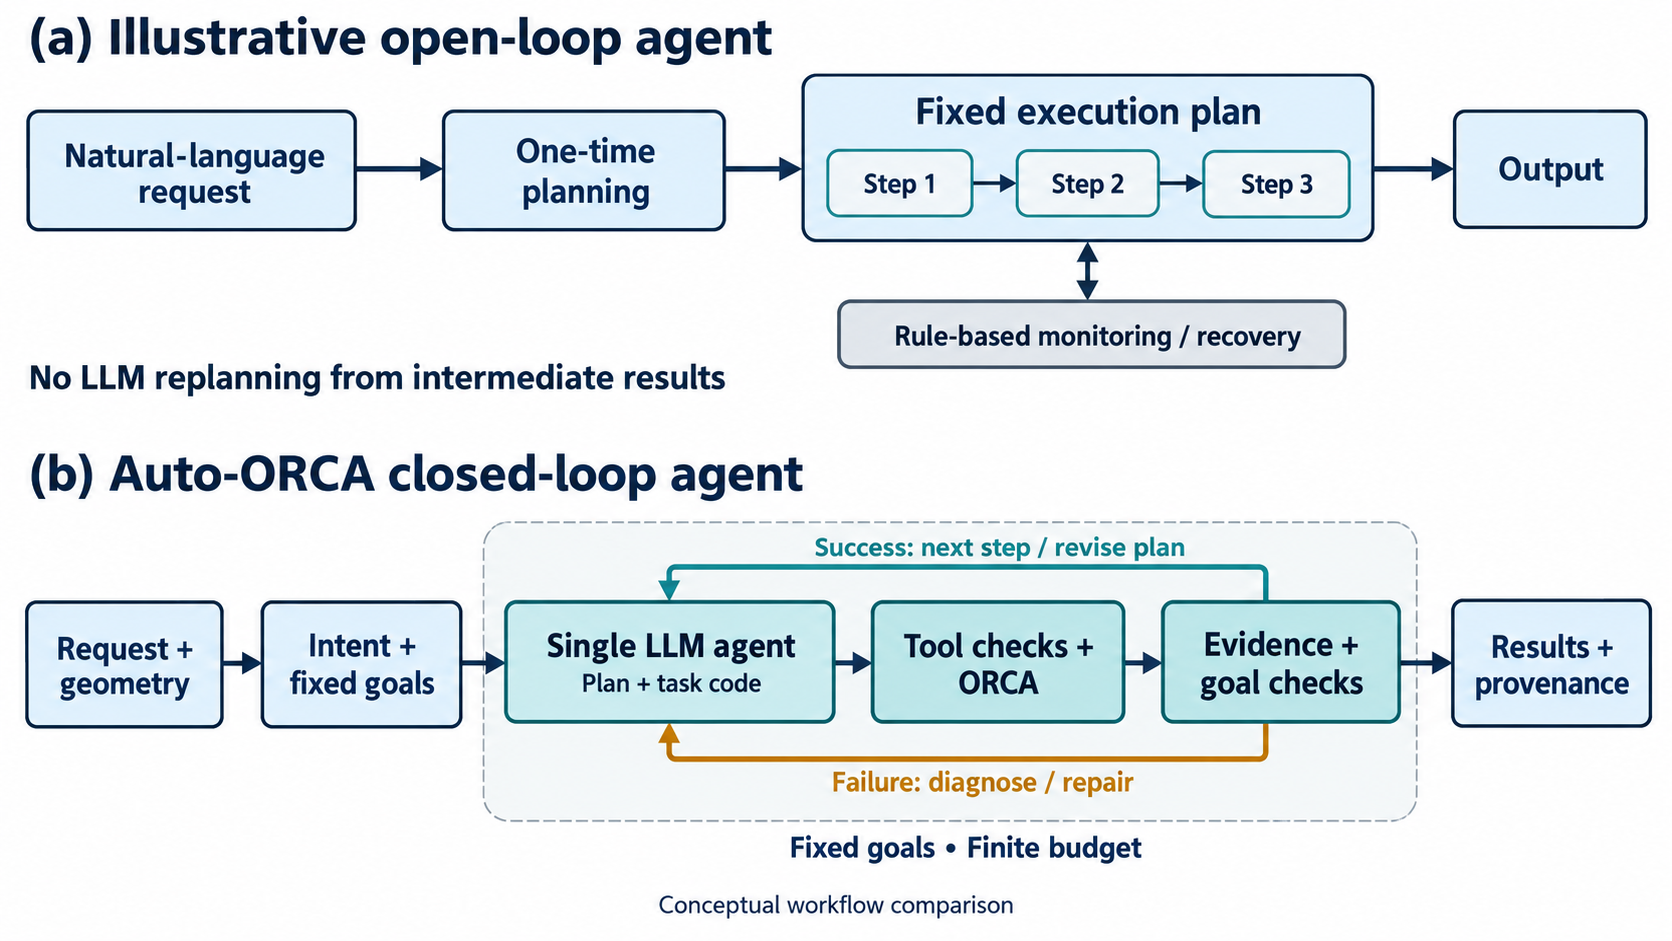
\includegraphics[width=\linewidth]{open-loop-vs-auto-orca.png}
  \caption{Comparison of the mechanisms underlying an open-loop agent and the Auto-ORCA closed-loop workflow.}
  \label{fig:open-closed-loop}
\end{figure}

In molecular calculations, later steps often require information available only after earlier steps have been completed.
For example, frequency analysis must be tied to the optimized structure actually obtained; conformer comparison requires identification of candidates with usable energies; and environmental comparisons require verification that the two calculations share a common geometry.
Returning this information to the decision process after execution allows plans to be grounded in evidence already obtained.
The Auto-ORCA closed loop therefore supports both exception handling and the use of successful results to advance the scientific investigation.

\begin{table}[htbp]
  \centering\small
  \caption{Mechanistic comparison of open-loop operation and Auto-ORCA.}
  \label{tab:loop-comparison}
  \begin{tabularx}{\linewidth}{>{\raggedright\arraybackslash}p{2.35cm}YY}
    \toprule
    Dimension & Illustrative open-loop agent & Auto-ORCA closed-loop organization\\
    \midrule
    Planning & Specifies the complete sequence and main parameters at the outset & Establishes an initial route and determines subsequent actions using new evidence\\
    Successful results & Supply inputs to predetermined steps and predefined post-processing & Also inform objective progress and the suitability of subsequent actions\\
    Exception handling & Monitors, retries, or stops according to predefined rules & Proposes checked repairs using diagnostics, previous attempts, and objectives\\
    Algorithm expression & Executes operations specified in the initial plan & Generates bounded task code for the problem and combines generic tools\\
    Condition preservation & Relies on the initial plan and execution rules & Stores original objectives independently and rechecks conditions after plan revisions\\
    Final delivery & Summarizes outputs from the executed route & Links results, actual conditions, provenance, and unresolved issues to each objective\\
    \bottomrule
  \end{tabularx}
\end{table}

The design advantage of Auto-ORCA lies in the explicit connection between decision-making and execution responsibilities.
A single agent continually addresses the same scientific objectives, generic tools implement each action, and raw artifacts provide a shared basis for subsequent decisions.
Computational, analytical, and interpretive requirements can thus be expressed within a unified task without constructing a separate complete workflow for every combination.
Combining an adaptable route with a stable problem definition provides a basis for gradual extension to more complex potential-energy-surface exploration.

\section{End-to-End Workflow from Natural Language to a Computational Report}
\label{sec:end-to-end-workflow}
Auto-ORCA progressively transforms a user's scientific question into an executable task with explicit inputs, computational conditions, and evidence sources.
The process can be summarized as natural-language input, intent recognition and condition confirmation, objective specification, planning with knowledge retrieval as needed, task code generation, ORCA execution, result checking and feedback, and final delivery.
The same agent loop coordinates these stages.
Because subsequent actions depend on facts already established, the actual route may include evidence queries, plan revisions, and supplementary analyses.
The following subsections describe how information passes between the stages.

\subsection{Natural-Language Input and Scientific Intent Recognition}
The task interface accepts natural-language descriptions together with user-provided structures, output files, or references to existing results.
The system first preserves the original request and identifies four types of information: the system to be studied, the physical quantities required, the conditions that the calculations must satisfy, and the materials the user expects to receive.
For example, ``optimize ethanol and calculate its vibrational frequencies'' must specify the molecular system, structure optimization, frequency calculation at the optimized structure, and delivery of the corresponding coordinates and numerical results.
``Compare the energies of the same structure in two environments'' additionally requires preservation of the common geometry and the pairing between the calculations.

Intent recognition produces a checkable structured candidate that records the system, objectives, geometric relationships, conditions, minimum evidence, and unresolved information.
Key fields retain their supporting source text.
The software checks the correspondence between this candidate and the user message before storing the normalized requirements.
Consequently, qualifiers such as ``the same geometry,'' ``the first five states,'' and ``the complete tensor'' can be preserved throughout the workflow, reducing the risk of recognizing only a broad task category while omitting delivery requirements.

\subsection{Condition Clarification and Objective Specification}
The method, basis set, charge, multiplicity, environment, and geometry source jointly define the actual computational problem.
The system distinguishes conditions explicitly supplied by the user, traceable inherited conditions, defaults, and authorized automatic choices.
Missing information remains recorded as unresolved.
The agent may ask targeted questions when an omission would change the system being calculated or the meaning of the result.
Where the user has delegated method or basis-set selection, the system may record a justified choice and check its compatibility with the remaining conditions before launching the calculation.

Once the conditions have been confirmed, the objectives and minimum evidence requirements are stored independently of the execution plan.
A request may contain multiple objectives, each with its own constraints on the system, environment, electronic state, and geometric relationships.
For example, a comparison of gas-phase and solution energies must preserve two environment-specific objectives and their common geometry; it cannot be reduced to an undifferentiated ``energy'' field.
Fixing the objectives preserves flexibility in the computational route: the plan may add parsing steps or repair inputs, but it must still address the original scientific question.

\subsection{On-Demand Knowledge Queries to Support Operations}
\label{sec:knowledge-retrieval}
When the next operation requires additional information on software syntax, methods, or property definitions, the agent formulates a specific query from the current uncertainty.
The query process comprises source selection, search-term formulation, retrieval of matching passages, and assessment of whether those passages support the current decision.
For example, preparing a frequency task may require consulting documentation on optimization and vibrational analysis; writing Python task code may require the interface documentation for the relevant OPI version; and diagnosing an input error may use the ORCA log to locate the relevant manual section.

Knowledge queries may also be used after results have been returned.
For example, references can help establish the meaning of physical quantities when explaining the relationship between nuclear magnetic shielding and chemical shifts or distinguishing electronic energy differences from free energies.
The numerical values, geometries, and convergence states of existing results are instead read from their corresponding raw artifacts.
The final report can therefore state the basis for an operation, the actual computational conditions, and the sources of its numerical results.

\subsection{Organizing the Computational Plan by Dependencies}
The agent next translates the objectives into interdependent operations, including reading or preparing structures, generating inputs, executing calculations, extracting properties, and organizing results.
Each step identifies the system to be used, the registered files it consumes, the tool it invokes, and the outputs it is expected to provide.
The software checks the relationship between the plan and the objectives, file dependencies, tool permissions, and available budgets.
An operation becomes eligible for execution only when its prerequisite data are available and satisfy the checks required by that step.

The plan translates scientific ordering requirements into data dependencies.
A frequency calculation after optimization must obtain the corresponding final structure; candidate energy ranking must preserve the association between each energy and its candidate identifier; and rotational consistency analysis requires results for two orientations together with the rotation definition.
When the route must change, the system creates a new plan version while preserving the original records of executed inputs and attempts.
This allows exploration to adapt to new information while retaining an explanation of the route that produced each result.

\subsection{Task Code Generation through a Unified Tool Boundary}
For tasks that are difficult to express directly through fixed interfaces, the agent may write Python task code and native ORCA input to perform repeated calculations, extract fields, organize matrices, or analyze deterministic derived quantities.
Code is first stored as a file with provenance and then referenced by an execution step.
Before execution, the system checks the identities of the code and inputs, file dependencies, and task declarations.
Generated programs run in a managed environment, and internal ORCA requests continue to pass through the unified entry point.

With this organization, new tasks are expressed primarily through changes in operation composition and task programs.
For example, conformer comparison requires managing a set of geometries and energies; excited-state analysis requires organizing state-resolved outputs; and shielding analysis requires preserving atom indices and matrix components.
All three can use the same mechanisms for file writing, execution, querying, and archiving.
Programs provide general computational capabilities, while the tool boundary maintains traceability of actual inputs, resource consumption, and raw artifacts.

\subsection{Execution, Monitoring, and Raw Artifact Archiving}
Before launch, the system verifies the actual inputs, geometry, conditions, permissions, and remaining resources, and creates a separate record for the operation.
Task code and its internal ORCA calculations share a controlled execution environment and cumulative resource constraints.
Launch is confirmed by a trusted execution receipt.
If the execution state is uncertain, existing processes and receipts are reconciled first, preventing an unknown state from being mistaken for a calculation that has not started and thereby duplicated.

After execution, the system archives inputs, standard output, error logs, structure files, and property files, and links each result to its raw artifacts.
Records are preserved for both normal completion and failure.
They provide specific objects for subsequent diagnosis and allow successful numerical results and failure causes to enter the same feedback process.

\subsection{Result Checking and Evidence-Based Continuation}
After receiving a new result, the main loop reevaluates the objectives before deciding on the next action.
Checks cover the actual conditions, file integrity, output readability, and applicable scientific validation.
Outputs covered by existing checks are evaluated according to their corresponding rules; new properties may be extracted by task code as observations with provenance, units, and validation statements.
Successful result reading, calculation completion, reportable observations, and verified scientific requirements are recorded separately so that final conclusions correspond to the evidence actually obtained.

Successful feedback may initiate a further necessary analysis.
For example, completed optimization must be followed by acquisition of the final structure and frequency evidence, while completed candidate calculations require consolidation of their associations and consistent energy units.
Failure feedback includes specific fields, program errors, or locations in ORCA logs so that the agent can propose targeted repairs.
When software documentation must be checked, the feedback can support a focused knowledge query whose findings inform the proposed revision.
Repairs use new inputs or subsequent steps while preserving the original objectives and sources that remain valid; the original failure remains accessible.

The system also checks whether executable work remains for the current objectives.
When approved subsequent steps, recoverable failures, or analytical routes based on archived originals remain available, feedback identifies the corresponding continuation options, and the final delivery check uses this information to prevent premature termination.
If existing files already support the required analysis, continuation may require only an additional parsing operation.
This mechanism connects calculation with analysis and directs further effort toward identified evidence gaps.

\subsection{Final Output and Verifiable Delivery}
When the task reaches a deliverable state, or when resources, permissions, or specific execution conditions require termination, the system consolidates the correspondence between objectives and evidence.
The final output includes the question and actual methods, the numerical results or structures obtained, necessary units and reference definitions, calculation and validation status, artifact locations, and outstanding work.
Method-selection rationales refer directly to saved records, while numerical values are traced to the corresponding raw outputs and analytical sources.
Knowledge sources used during the task are linked through retrieval records to document versions and passage locations, preserving traceability of both the operational rationale and the result sources.

For the user, this delivery provides a continuous path from posing a question to obtaining computational materials suitable for further use.
Tables facilitate comparison, raw files support verification, and limitations indicate what additional evidence is needed.
The calculation success rate used in this report describes whether corresponding ORCA calculations for the seven questions completed normally and produced numerical results.
The scientific conclusions supported by each result remain separately delimited by its method, geometry, and property evidence.

\subsection{Illustration: Information Flow in Ethanol Optimization and Frequency Analysis}
Using ethanol optimization and vibrational frequency analysis as an illustrative example, the table below traces the information flow from a natural-language request to final delivery.

\begin{table}[htbp]
  \centering\small
  \caption{Progressive specification of information in the ethanol task.
  The illustrative natural-language input is ``Optimize neutral singlet ethanol in the gas phase using r$^{2}$SCAN-3c and report its vibrational frequencies.''}
  \label{tab:workflow-example}
  \begin{tabularx}{\linewidth}{>{\raggedright\arraybackslash}p{2.35cm}YY}
    \toprule
    Stage & Information established & Information passed to the next stage\\
    \midrule
    Intent recognition & Ethanol; structure optimization; vibrational frequencies & Two types of results and the requirement to calculate frequencies at the optimized structure\\
    Condition confirmation & Gas phase, neutral singlet, r$^{2}$SCAN-3c & Confirmed method, built-in basis set, and geometry source\\
    On-demand knowledge queries & Relevant references on the method, interface, or frequency settings & Citable source passages, software versions, and operational rationale\\
    Planning & Structure preparation, calculation, extraction, and interpretation & Inputs and required outputs for each operation\\
    Code and input & Actual ORCA input and any required analysis programs & File identities, conditions, and resource declarations\\
    Execution and archiving & Raw outputs, final coordinates, and property files & Actual completion status and readable artifacts\\
    Checking and analysis & Convergence records, mode count, and imaginary frequencies & Evidence concerning energy, frequencies, and local stability\\
    Result delivery & Methods, numerical values, coordinates, and interpretation & Readable conclusions and computational materials available for further use\\
    \bottomrule
  \end{tabularx}
\end{table}
